\documentclass[ignorenonframetext,]{beamer}
\setbeamertemplate{caption}[numbered]
\setbeamertemplate{caption label separator}{: }
\setbeamercolor{caption name}{fg=normal text.fg}
\beamertemplatenavigationsymbolsempty
\usepackage{lmodern}
\usepackage{amssymb,amsmath}
\usepackage{ifxetex,ifluatex}
\usepackage{fixltx2e} % provides \textsubscript
\ifnum 0\ifxetex 1\fi\ifluatex 1\fi=0 % if pdftex
  \usepackage[T1]{fontenc}
  \usepackage[utf8]{inputenc}
\else % if luatex or xelatex
  \ifxetex
    \usepackage{mathspec}
  \else
    \usepackage{fontspec}
  \fi
  \defaultfontfeatures{Ligatures=TeX,Scale=MatchLowercase}
\fi
% use upquote if available, for straight quotes in verbatim environments
\IfFileExists{upquote.sty}{\usepackage{upquote}}{}
% use microtype if available
\IfFileExists{microtype.sty}{%
\usepackage{microtype}
\UseMicrotypeSet[protrusion]{basicmath} % disable protrusion for tt fonts
}{}
\newif\ifbibliography
\hypersetup{
            pdftitle={Introducción a R},
            pdfauthor={Inteligencia de Negocios},
            pdfborder={0 0 0},
            breaklinks=true}
\urlstyle{same}  % don't use monospace font for urls

% Prevent slide breaks in the middle of a paragraph:
\widowpenalties 1 10000
\raggedbottom

\AtBeginPart{
  \let\insertpartnumber\relax
  \let\partname\relax
  \frame{\partpage}
}
\AtBeginSection{
  \ifbibliography
  \else
    \let\insertsectionnumber\relax
    \let\sectionname\relax
    \frame{\sectionpage}
  \fi
}
\AtBeginSubsection{
  \let\insertsubsectionnumber\relax
  \let\subsectionname\relax
  \frame{\subsectionpage}
}

\setlength{\parindent}{0pt}
\setlength{\parskip}{6pt plus 2pt minus 1pt}
\setlength{\emergencystretch}{3em}  % prevent overfull lines
\providecommand{\tightlist}{%
  \setlength{\itemsep}{0pt}\setlength{\parskip}{0pt}}
\setcounter{secnumdepth}{0}

\title{Introducción a R}
\subtitle{Lenguaje R}
\author{Inteligencia de Negocios}
\date{16 agosto 2018}

\begin{document}
\frame{\titlepage}

\begin{frame}{Introducción}

\begin{center}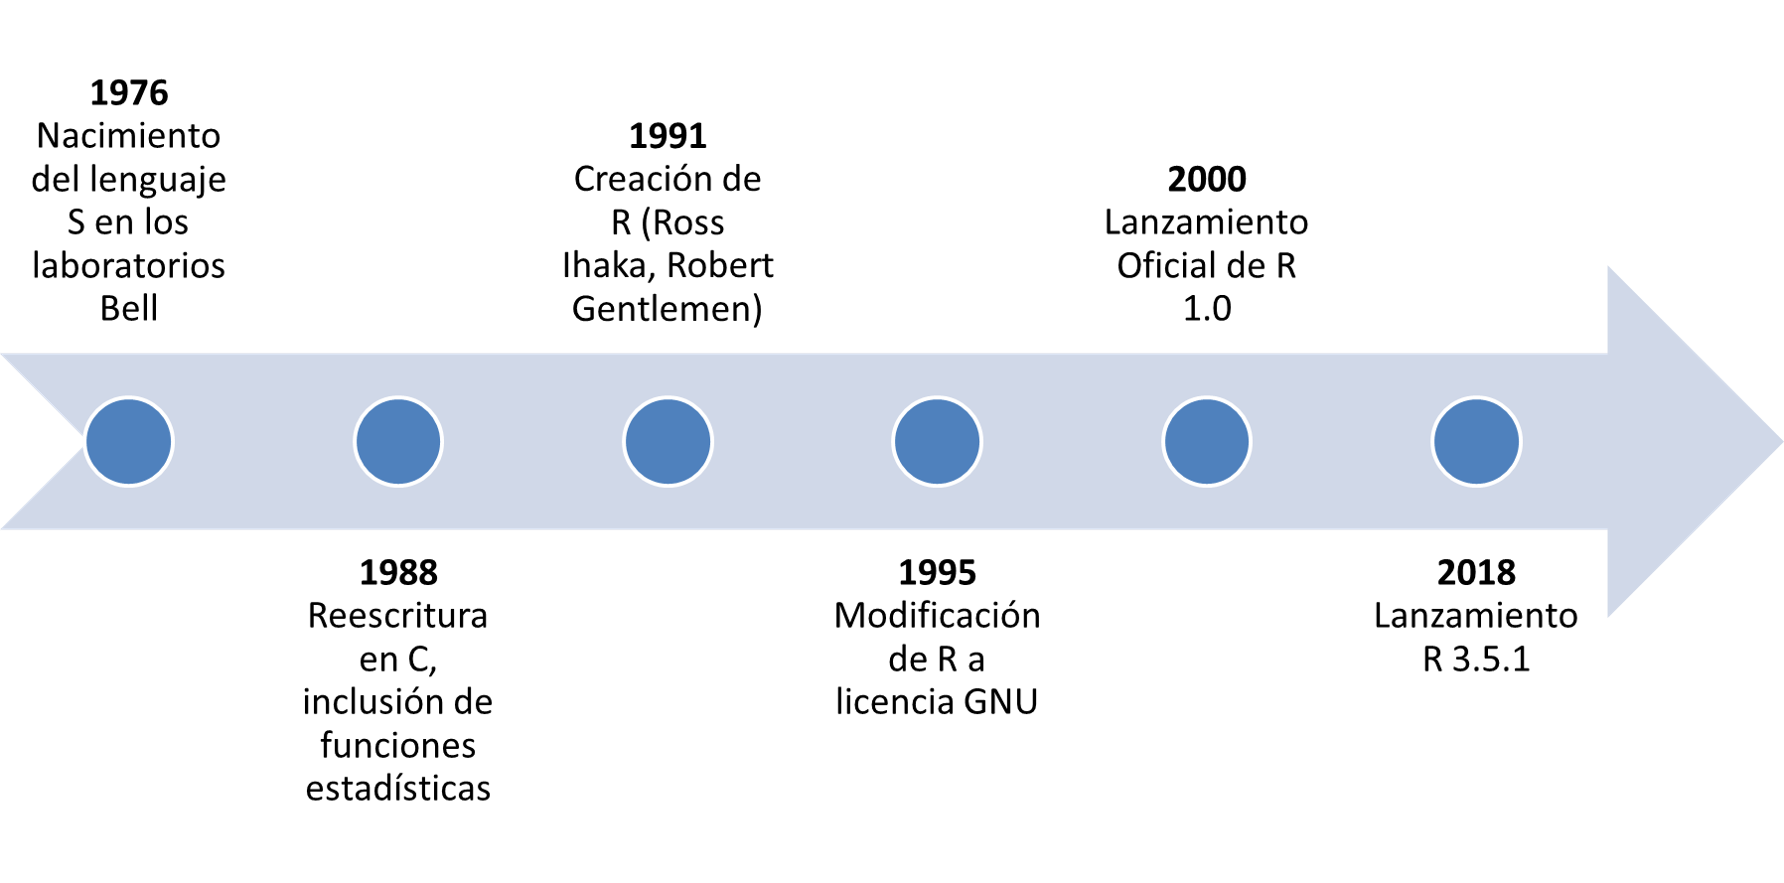
\includegraphics[width=1000px]{./img/img1} \end{center}

\end{frame}

\begin{frame}{Instalación}

El software puede ser descargado de
\href{https://cran.r-project.org/bin/windows/base/R-3.5.1-win.exe}{aqui}.

Una vez se cuenta con el software se procede a descarad un IDE
(Integrated Development Environment)
\href{https://www.rstudio.com/products/rstudio/download/\#download}{R
Studio}.

Este último permite escribir y ejecutar código, a la vez que cuenta con
interfaces que facilitan ciertos procesos

\end{frame}

\begin{frame}{Interfaz}

\begin{center}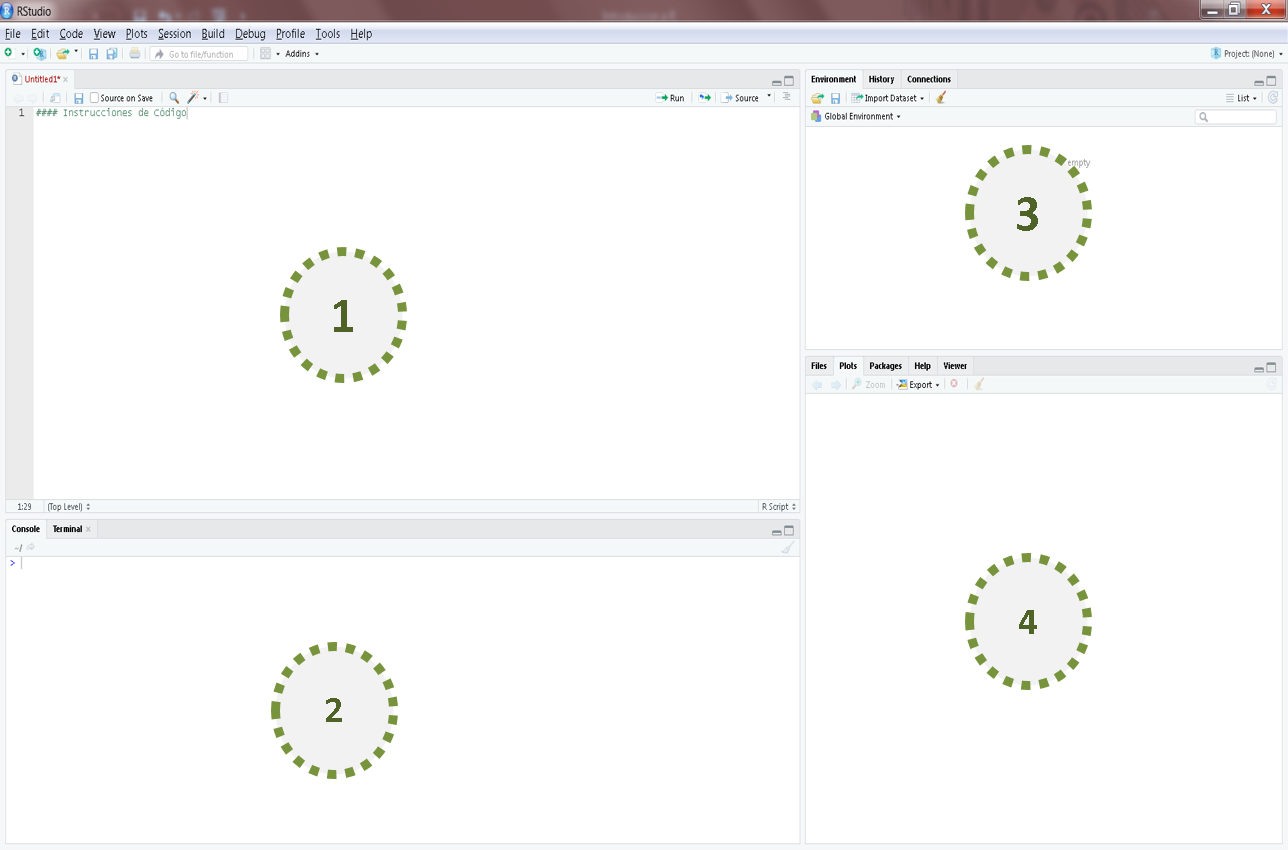
\includegraphics[width=800px]{./img/img2} \end{center}

\end{frame}

\begin{frame}{Opciones de Usuario}

\begin{center}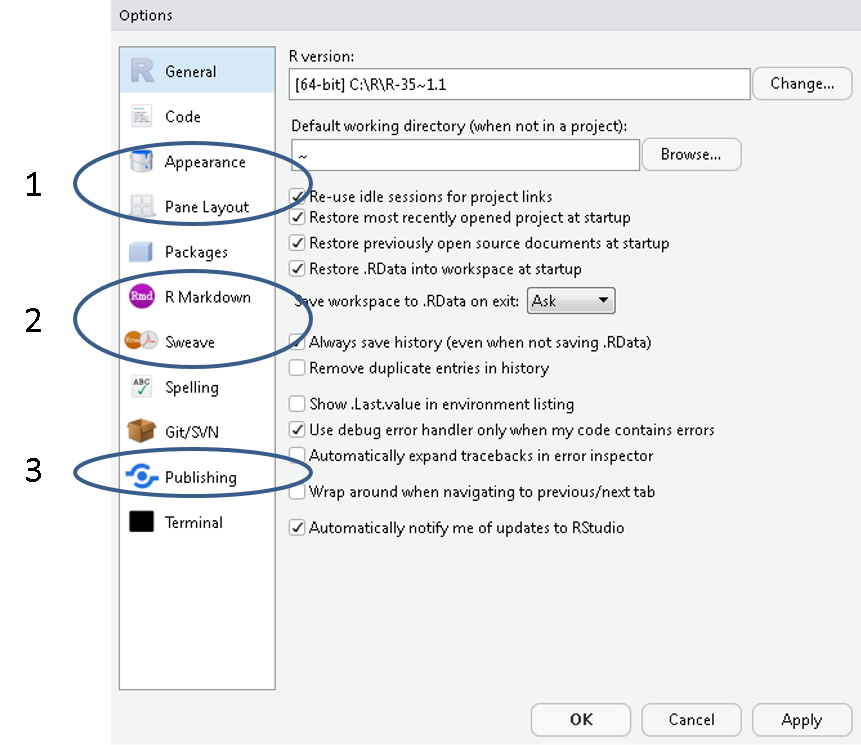
\includegraphics[width=500px]{./img/img3} \end{center}

\end{frame}

\begin{frame}{Paquetes}

Los paquetes \emph{``base''} son cargados por defecto al momento de
iniciar una sesión

Hay 29 paquetes suministrados con R (llamados paquetes ``estándares'' y
``recomendados''.

Muchos (muchos) más están disponibles para ser instalados a través de
\href{http://CRAN.R-project.org}{CRAN}

\end{frame}

\begin{frame}{CRAN}

The Comprehensive R Archive Network (CRAN) es el repositorio de los
paquetes aprobados por R

Existen otros repositorios de los cuales se pueden instalar paquetes:

\begin{itemize}
\tightlist
\item
  Bioconductor.
\item
  Github.
\item
  Etc.
\end{itemize}

\begin{center}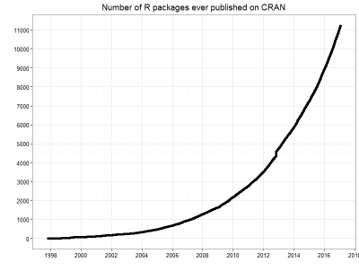
\includegraphics[width=380px]{./img/img4} \end{center}

\end{frame}

\begin{frame}{Instalación de Paquetes}

Según el Repositorio del que se desea instalar la instrucción cambia e
incluso puede depender de otros paquetes.

Adicionalmente R-Studio ofrece la interfaz de instalación de paquetes

Todo paquete debe ser cargado al ambiente de trabajo. Cada vez que se
abre una sesión es necesario cargar los paquetes

\end{frame}

\begin{frame}[fragile]{Ayudas}

\begin{itemize}
\item
  Supongamos que queramos conocer sobre la función \texttt{mean} de R
  \texttt{?mean} o \texttt{help(mean)} abren la pagina de ayuda sobre la
  función.
\item
  \texttt{??mean} realiza una búsqueda por palabras clave en el help.
\item
  Hay muchas comunidades de discusión y foros sobre los problemas
  típicos que los usuarios encuentran usando R Por ejemplo:
\item
  \href{http://stackoverflow.com/}{StackOverflow}
\item
  \href{https://r-dir.com/community/forums.html}{R Dir}
\item
  En general, muchas preguntas que se puedan tener ya tienen respuesta
  en Internet.
\end{itemize}

\end{frame}

\begin{frame}{Ambiente de Trabajo}

El directorio de trabajo es por defecto el folder ``Home''

La carpeta \emph{``Home''} es modificable desde las opciones de usuario.

Es posible cambiar el directorio de trabajo en cada sesión.

La creación de un proyecto permite asignar directorios de trabajo de una
manera integrada

Una vez se establezca el directorio de trabajo, es posible navegar por
los archivos desde R-Studio

\end{frame}

\begin{frame}{Paquetes Recomendados:}

\begin{itemize}
\tightlist
\item
  dplyr : Manipulación de Dataframes
\item
  tidyr : Data Wrangling.
\item
  Rcmdr : Interfaz gráfica para ciertas tareas de R
\item
  data.table: Manipulación de Dataframes
\item
  ggplot2 : Gráficos estilizados
\item
  forecast: Pronósticos de datos temporales
\item
  agricolae: Paquete especializado en diseños de experimentos
\item
  shiny : Creación de Dashboards
\item
  Un largo etc.
\end{itemize}

\end{frame}

\end{document}
